\documentclass[11pt,a4paper,oneside]{report}

% ==========================================
% PACKAGES & CONFIGURATION
% ==========================================
\usepackage[utf8]{inputenc}
\usepackage[T1]{fontenc}
\usepackage[margin=1in]{geometry}
\usepackage{graphicx}
\usepackage{xcolor}
\usepackage{hyperref}
\usepackage{booktabs}
\usepackage{listings}
\usepackage{float}
\usepackage{titlesec}
\usepackage{caption}
\usepackage{subcaption}
\usepackage{fancyhdr}
\usepackage{amsmath}
\usepackage{amssymb}
\usepackage{enumitem}
\usepackage{longtable}
\usepackage{array}
\usepackage{etoolbox}

% Colors
\definecolor{navy}{HTML}{003875}
\definecolor{skyblue}{HTML}{378ADD}
\definecolor{codegray}{rgb}{0.5,0.5,0.5}
\definecolor{codepurple}{rgb}{0.58,0,0.82}
\definecolor{backcolour}{rgb}{0.95,0.95,0.92}

% Code Style
\lstdefinestyle{pythonstyle}{
    backgroundcolor=\color{backcolour},   
    commentstyle=\color{codegray},
    keywordstyle=\color{navy},
    numberstyle=\tiny\color{codegray},
    stringstyle=\color{codepurple},
    basicstyle=\ttfamily\footnotesize,
    breakatwhitespace=false,         
    breaklines=true,                 
    captionpos=b,                    
    keepspaces=true,                 
    numbers=left,                    
    numbersep=5pt,                  
    showspaces=false,                
    showstringspaces=false,
    showtabs=false,                  
    tabsize=2
}
\lstset{style=pythonstyle}

% Header/Footer
\pagestyle{fancy}
\fancyhf{}
\rhead{\color{navy}AI Job Market Intelligence}
\lhead{Group 8 | FAST-NUCES}
\rfoot{Page \thepage}

% Title Spacing
\titleformat{\chapter}[display]
  {\normalfont\bfseries\color{navy}}
  {\filleft\Large\chaptertitlename\ \thechapter}
  {1ex}
  {\titlerule\vspace{1ex}\filleft\Huge}

\hypersetup{
    colorlinks=true,
    linkcolor=navy,
    filecolor=magenta,      
    urlcolor=skyblue,
    pdftitle={AI Job Market Intelligence: Final Project Report},
}

% ==========================================
% TITLE PAGE
% ==========================================
\begin{document}

\begin{titlepage}
    \centering
    \vspace*{1cm}
    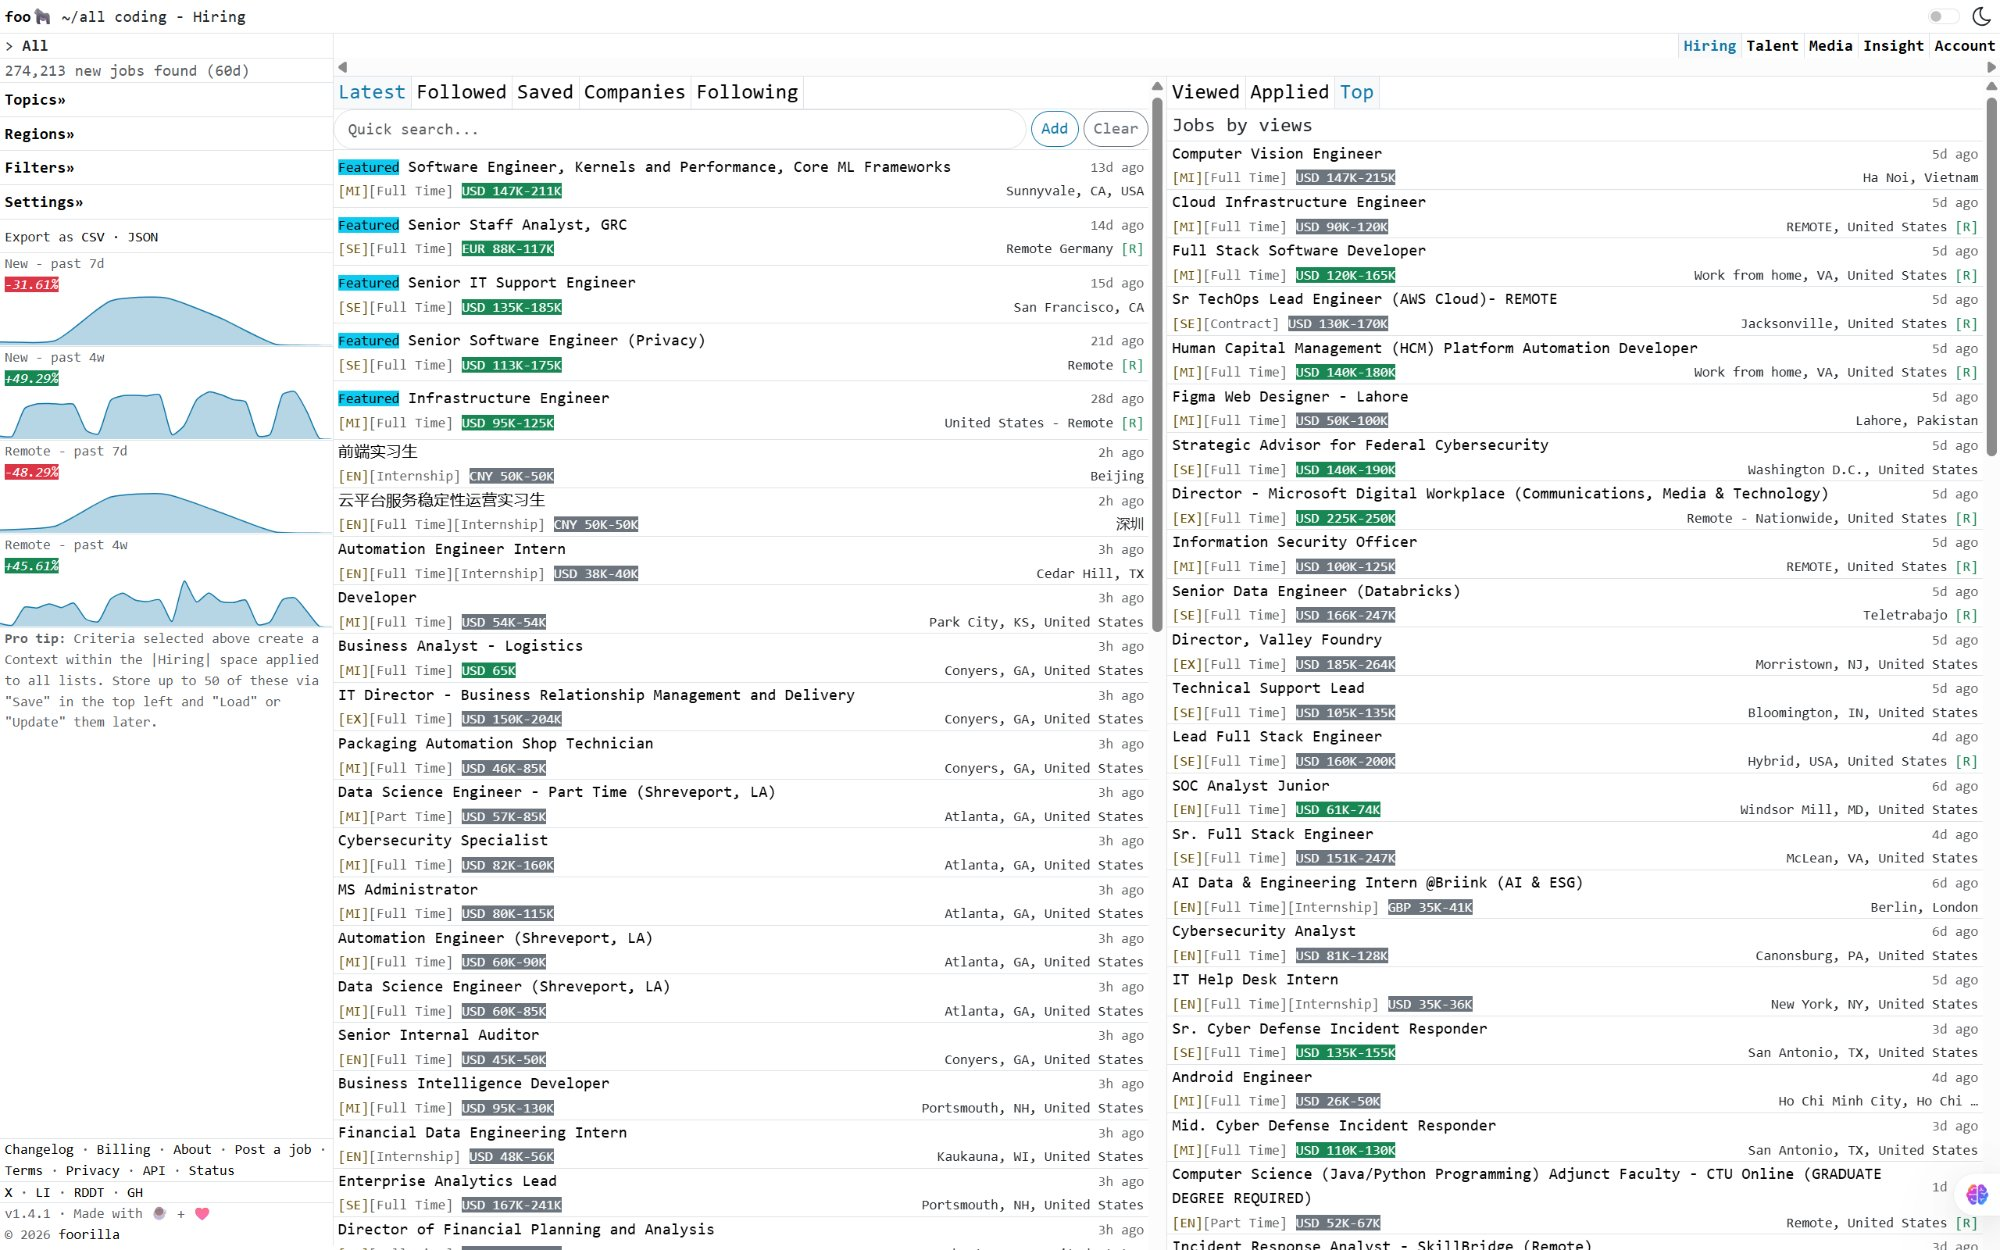
\includegraphics[width=0.4\textwidth]{../assets/pic1_foorilla_hiring.png}\\[1cm] % Placeholder for logo if available, or just a project-related image
    {\Huge \textbf{\color{navy}AI Job Market Intelligence}} \\[0.5cm]
    {\Large \textit{Salaries, Roles \& Global Hiring Trends (2020--2025)}} \\[1.5cm]
    
    {\large \textbf{CS3012: Fundamentals of Data Visualization}} \\[0.2cm]
    {\large Final Project Report} \\[2cm]
    
    \textbf{Prepared by Group 8:} \\[0.5cm]
    \begin{table}[H]
        \centering
        \begin{tabular}{ll}
            \textbf{Muhammad Nouman Hafeez} & \textbf{I210416} \\
            \textbf{M. Asim} & \textbf{I210852} \\
            \textbf{Sara Jabeen} & \textbf{I210624} \\
        \end{tabular}
    \end{table}
    
    \vfill
    
    \textbf{Instructor:} \\[0.2cm]
    {\large Dr. Atif Mughees} \\[1cm]
    
    \textbf{Department of Computer Science} \\
    \textbf{FAST-NUCES Islamabad} \\
    \textbf{Spring 2026}
\end{titlepage}

% ==========================================
% PRELIMINARIES
% ==========================================
\pagenumbering{roman}

\chapter*{Abstract}
This report details the comprehensive development of the "AI Job Market Intelligence" project, an end-to-end data visualization initiative aimed at uncovering the dynamics of the global Artificial Intelligence, Machine Learning, and Data Science labor markets. Utilizing a real-world crowdsourced dataset of over 150,000 records, the project implements a rigorous data science workflow—from exploratory data analysis and Python-based preprocessing to the engineering of 12 analytical features. The culmination is an interactive Tableau dashboard that provides high-fidelity insights into salary growth, the shift in remote work paradigms, and geographic compensation disparities. This document serves as a complete technical reference for the project's methodology, implementation, and findings.

\tableofcontents
\listoffigures
\listoftables

\newpage
\pagenumbering{numeric}

% ==========================================
% CHAPTER 1: INTRODUCTION
% ==========================================
\chapter{Introduction}

\section{Background}
The rapid advancement of Artificial Intelligence and Machine Learning has transformed the global tech industry, leading to a surge in demand for specialized talent. As organizations integrate AI into their core operations, the roles of Data Scientists, ML Engineers, and Data Architects have become pivotal. However, for both job seekers and hiring managers, navigating the compensation landscape is challenging due to the high variance in pay across regions, experience levels, and specific sub-disciplines.

\section{Problem Statement}
While various job boards provide salary data, most lack the granularity and historical context needed to understand long-term trends, especially the recent shift from pandemic-induced remote work back to on-site operations. Furthermore, raw crowdsourced data often contains noise, inconsistencies, and extreme outliers that can misguide analysis if not handled with precise statistical cleaning.

\section{Project Objectives}
The primary goals of this project are:
\begin{itemize}
    \item To clean and standardize a raw dataset of 150,000+ AI salary submissions.
    \item To engineer meaningful analytical dimensions (e.g., salary bands, regional groupings).
    \item To build an interactive, production-grade Tableau dashboard.
    \item To provide data-driven answers to key industry questions regarding career progression and the "remote work collapse."
\end{itemize}

\section{Core Research Questions}
The visualization and analysis aim to address the following:
\begin{enumerate}
    \item \textbf{Compensation Leadership:} Which specialized AI roles command the highest premiums?
    \item \textbf{Experience Premium:} What is the mathematical ratio between entry-level and executive-level earnings?
    \item \textbf{Remote Work Dynamics:} How has the percentage of remote work shifted year-over-year from 2022 to 2025?
    \item \textbf{Geographic Hubs:} Which countries lead in volume, and how does the "Rest of World" compare to the United States in terms of average pay?
    \item \textbf{Market Distribution:} How are salaries distributed across pay bands and quartiles?
\end{enumerate}

% ==========================================
% CHAPTER 2: DATA ACQUISITION & VERIFICATION
% ==========================================
\chapter{Data Acquisition \& Verification}

\section{Source Description}
The project leverages the "Global Salaries in AI, ML, Data Science and Big Data" dataset. This is a first-party release by \textit{aijobs.net} (owned by foorilla.com), published under the CC0 1.0 Public Domain license.

\section{Data Verification}
To ensure the authenticity of the dataset, we cross-referenced the Kaggle release with the live hiring platforms. The following assets demonstrate the source's operational presence in the market.

\begin{figure}[H]
    \centering
    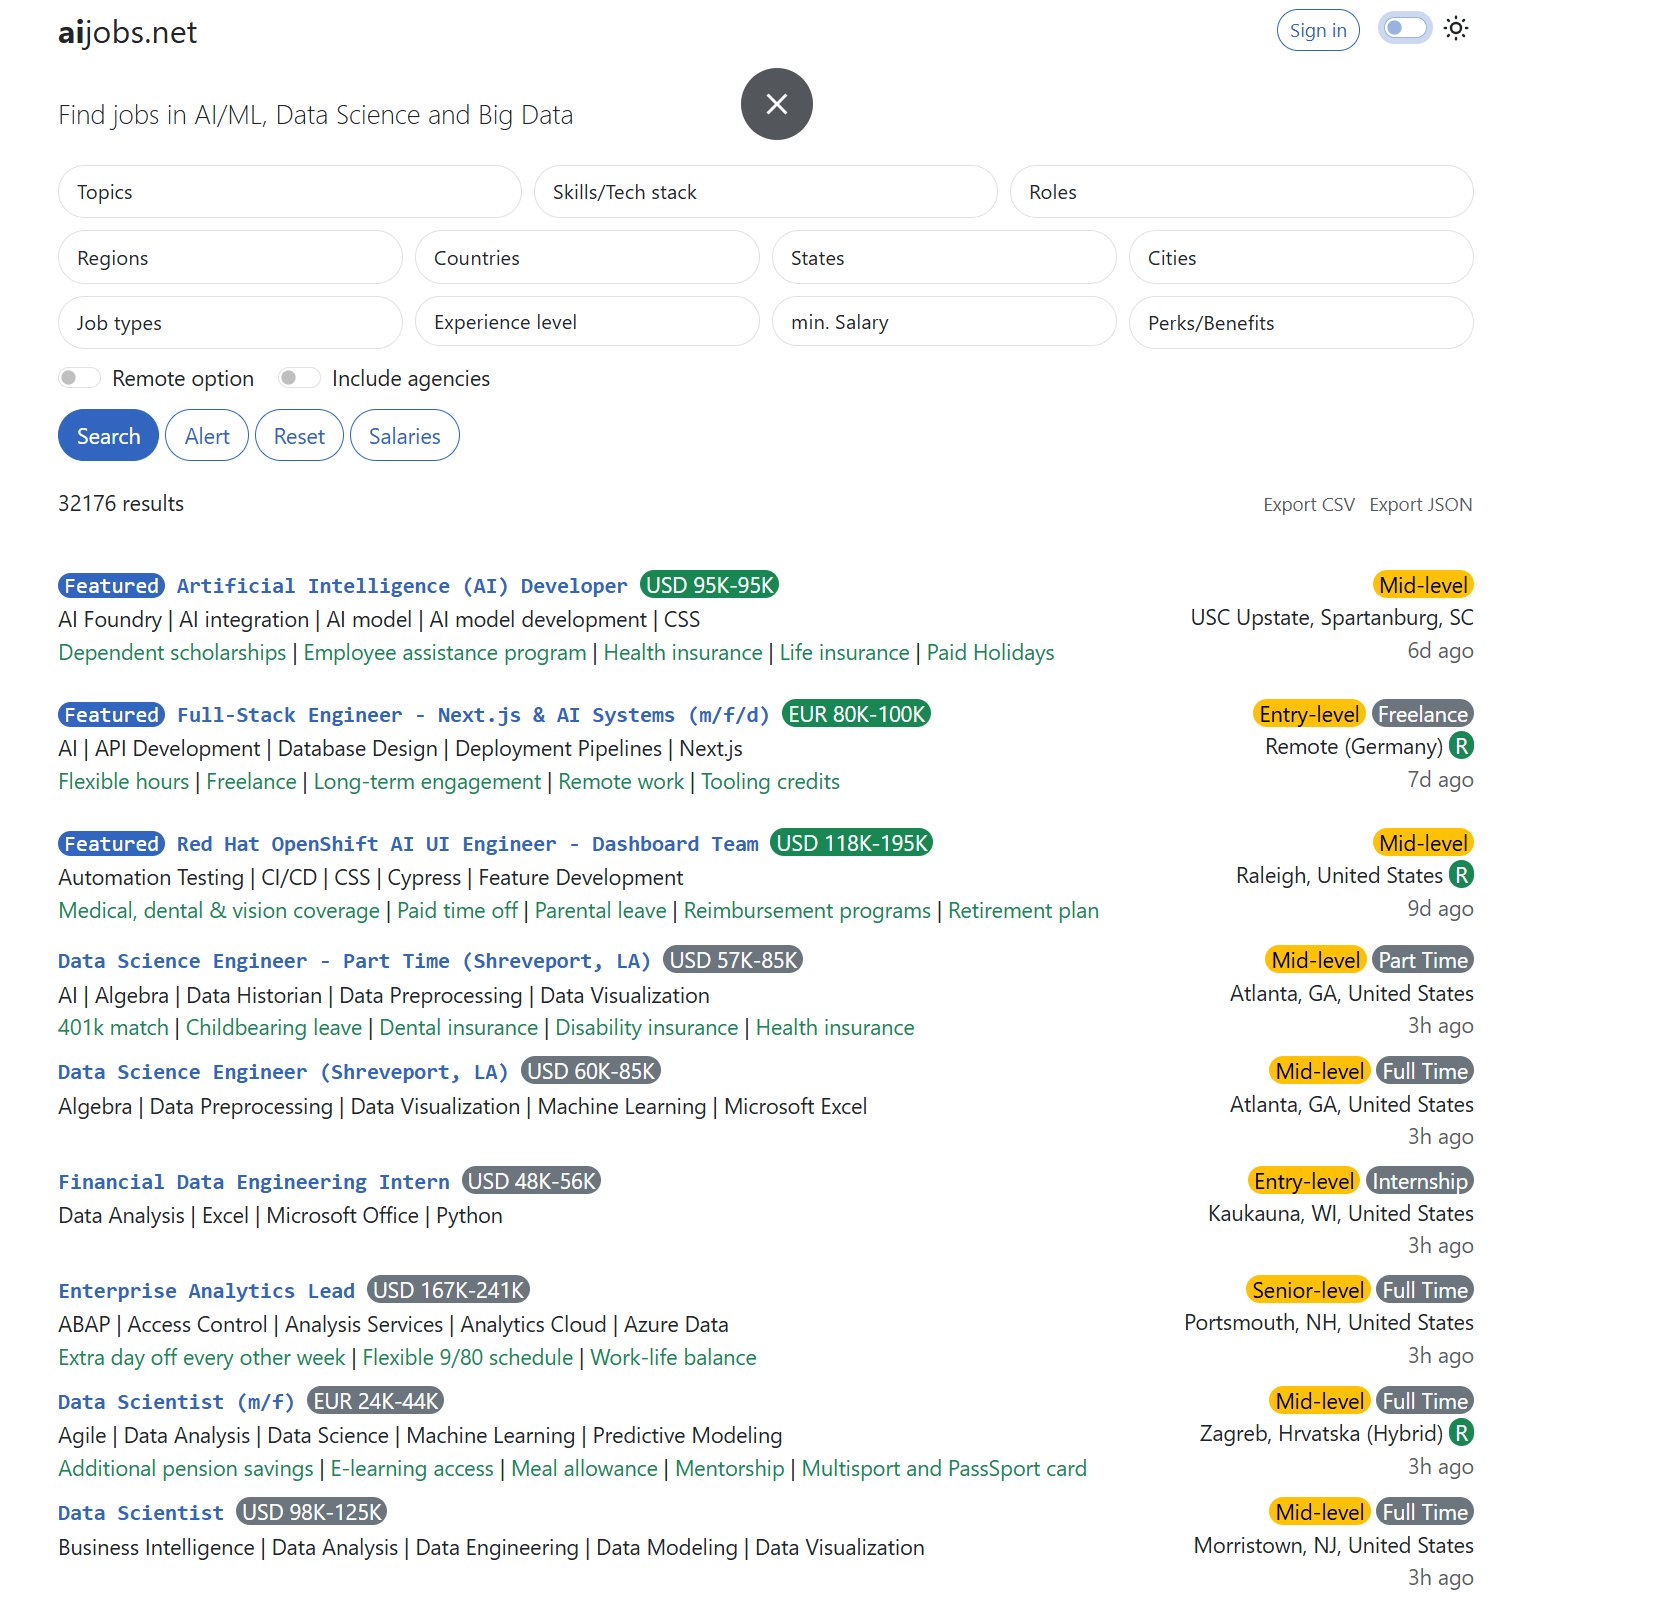
\includegraphics[width=0.8\textwidth]{../assets/pic4_aijobs_search.png}
    \caption{aijobs.net Search Interface - Source of Crowdsourced Data}
    \label{fig:asset_aijobs}
\end{figure}

\begin{figure}[H]
    \centering
    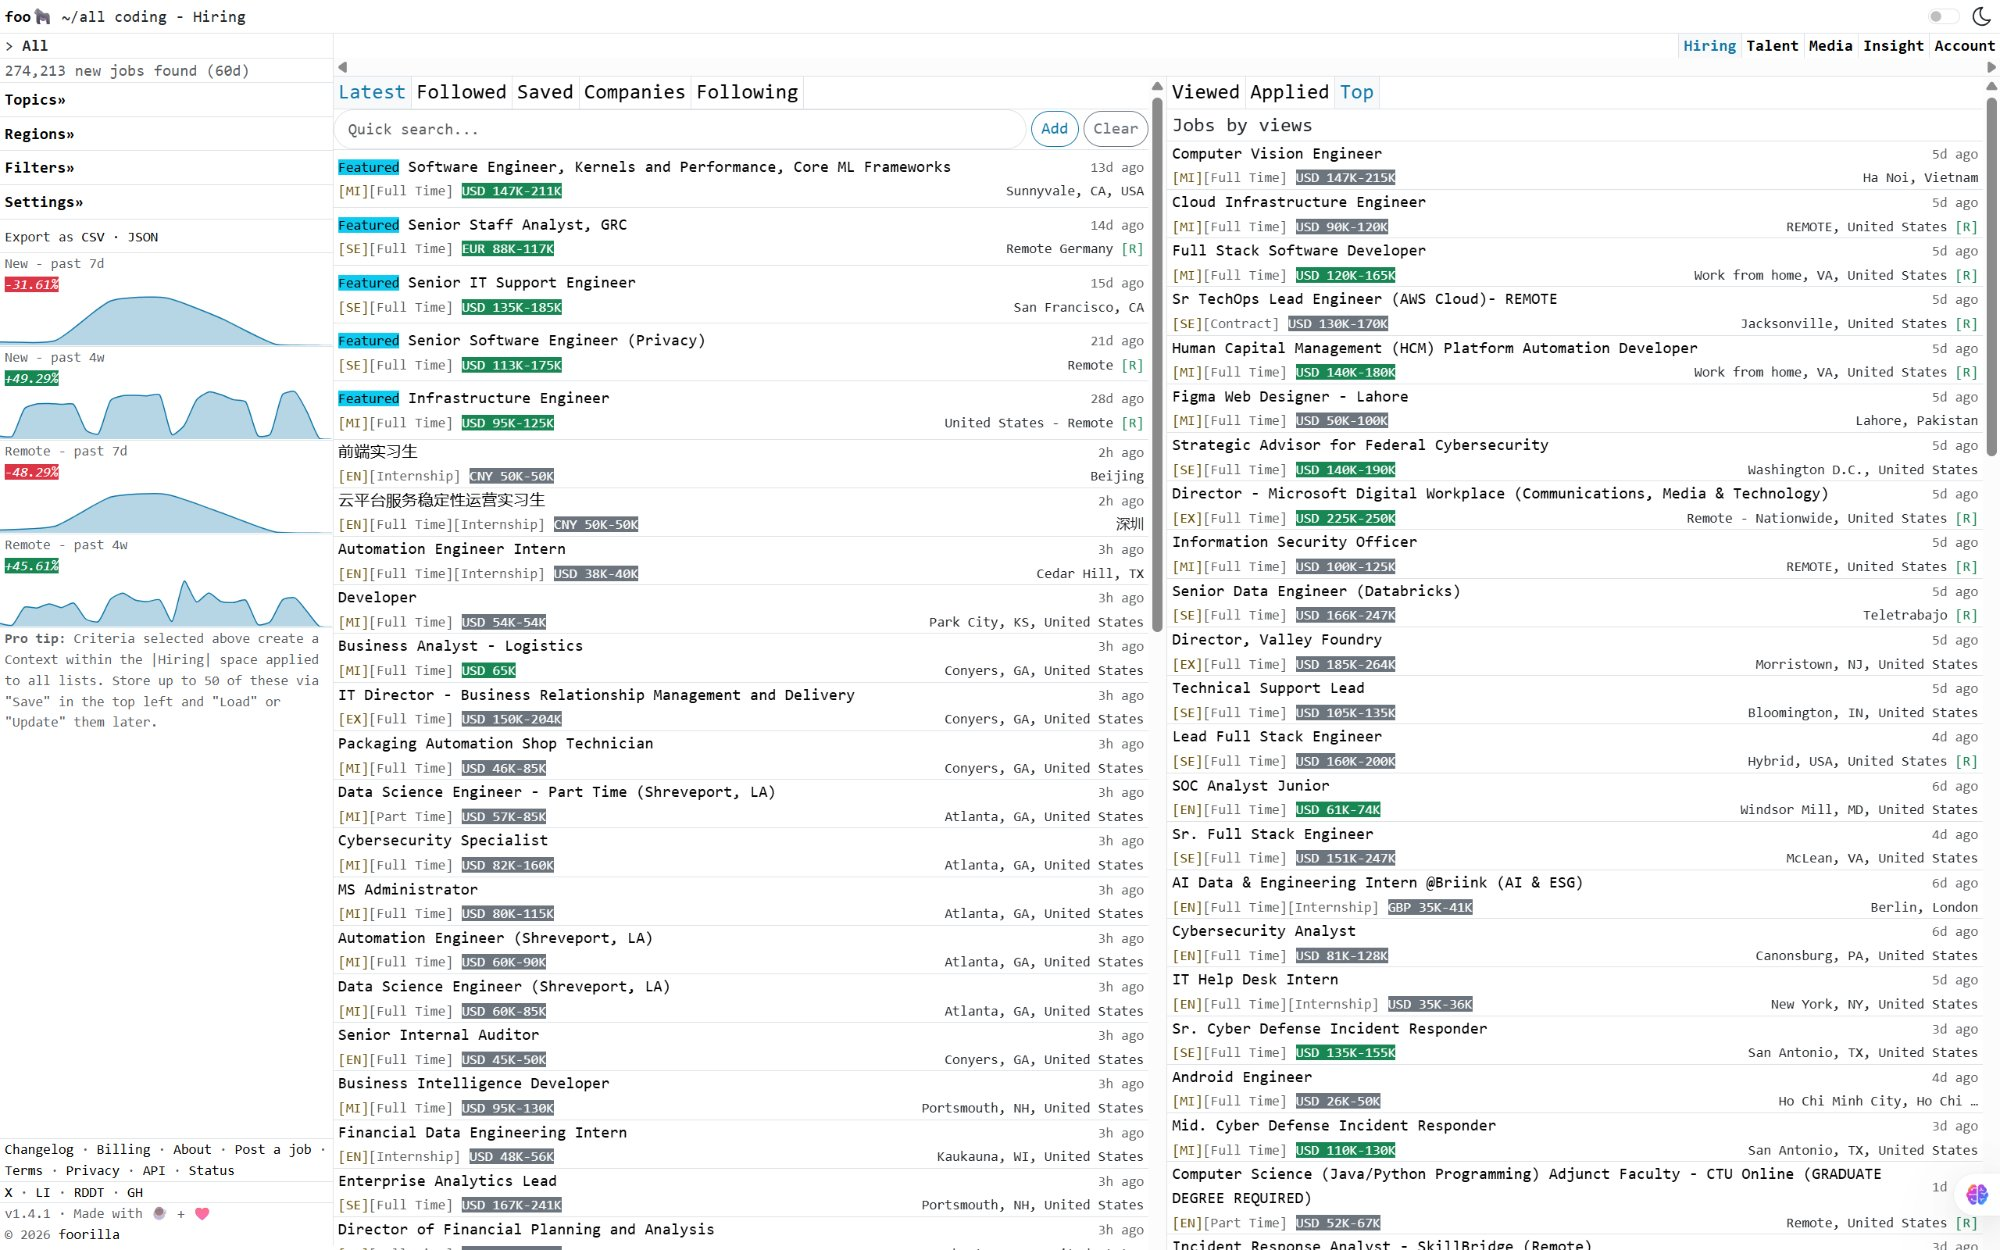
\includegraphics[width=0.8\textwidth]{../assets/pic1_foorilla_hiring.png}
    \caption{Foorilla Platform - Data Aggregation and Hiring Insights}
    \label{fig:asset_foorilla}
\end{figure}

\begin{figure}[H]
    \centering
    \begin{subfigure}[b]{0.48\textwidth}
        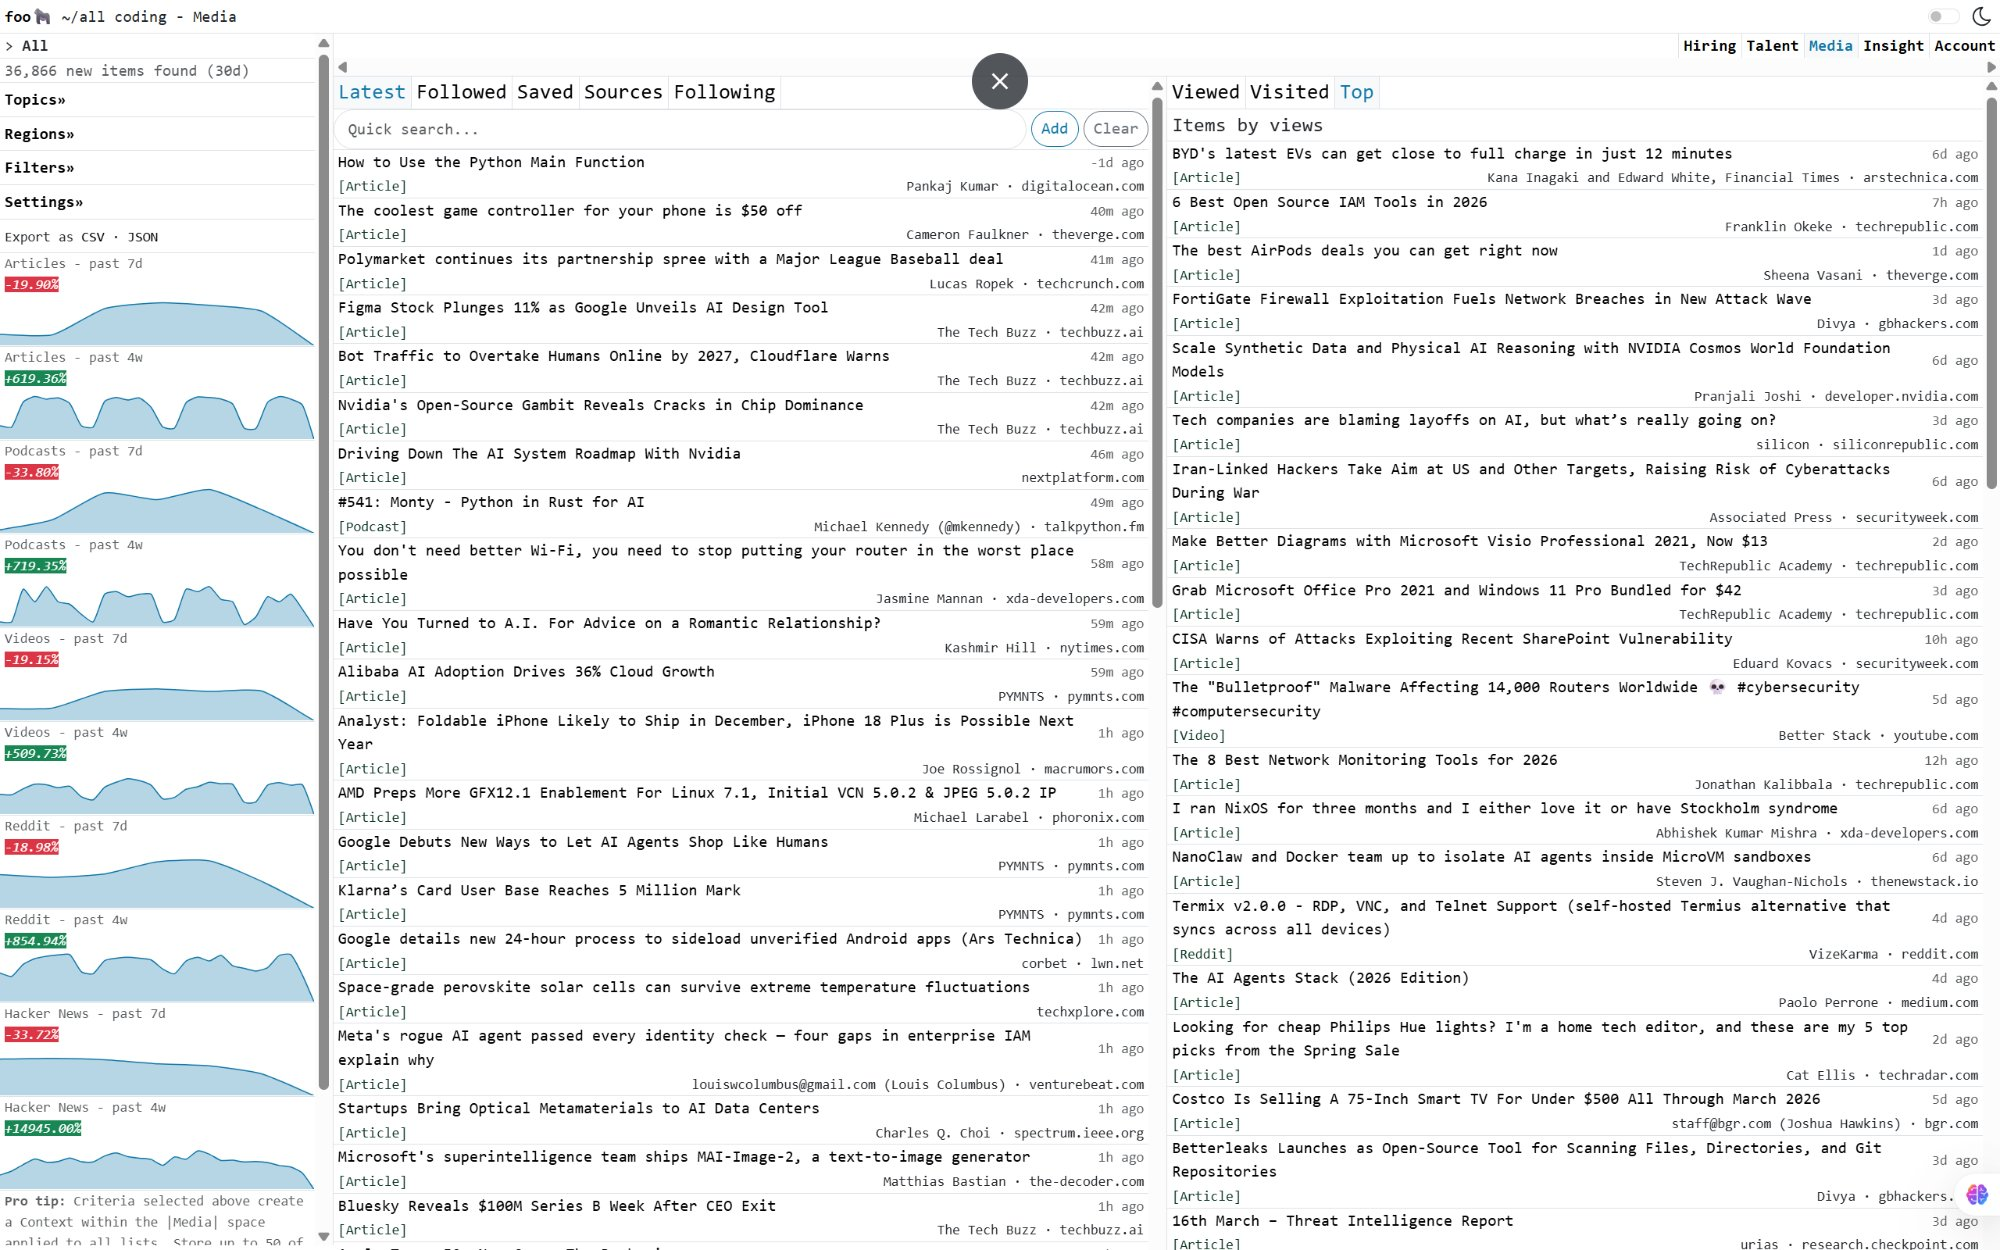
\includegraphics[width=\textwidth]{../assets/pic2_foorilla_media.png}
        \caption{Foorilla Media Presence}
    \end{subfigure}
    \hfill
    \begin{subfigure}[b]{0.48\textwidth}
        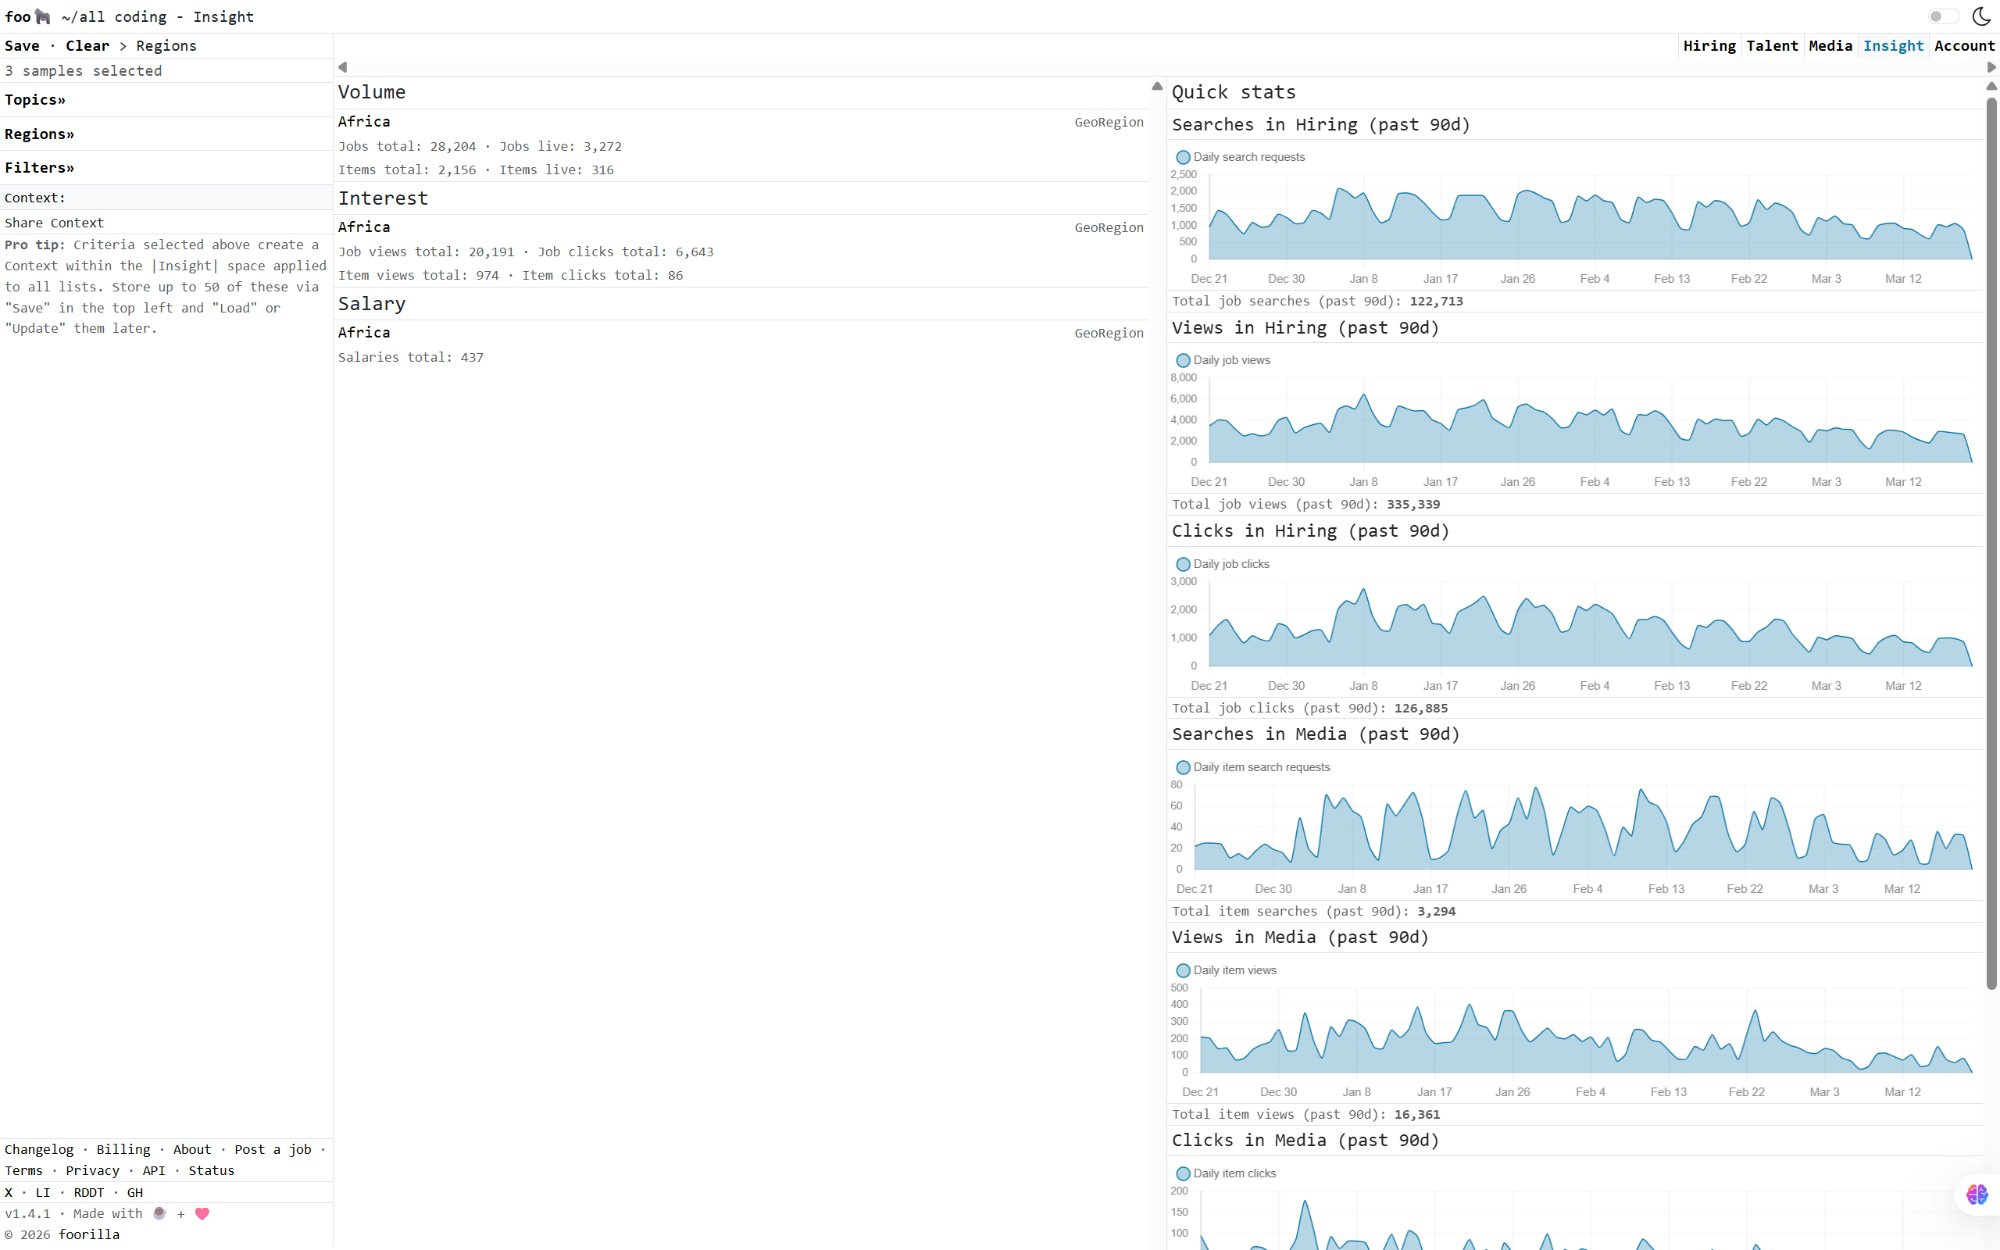
\includegraphics[width=\textwidth]{../assets/pic3_foorilla_insight.png}
        \caption{Foorilla Market Insights}
    \end{subfigure}
    \caption{Source Platform Verification Assets}
\end{figure}

\section{Initial Schema}
The raw dataset consists of 11 core columns as shown in Table \ref{tab:raw_schema}.

\begin{table}[H]
    \centering
    \caption{Raw Dataset Column Reference}
    \label{tab:raw_schema}
    \begin{tabular}{lp{10cm}}
        \toprule
        \textbf{Column} & \textbf{Description} \\
        \midrule
        work\_year & The year the salary was paid (2020--2025). \\
        experience\_level & EN (Entry), MI (Mid), SE (Senior), EX (Executive). \\
        employment\_type & FT (Full-time), PT (Part-time), CT (Contract), FL (Freelance). \\
        job\_title & The raw job title string (e.g., "Sr. Data Scientist"). \\
        salary & The raw salary amount in local currency. \\
        salary\_currency & The ISO 4217 currency code. \\
        salary\_in\_usd & The salary converted to USD (primary measure). \\
        employee\_residence & The employee's country of residence (ISO code). \\
        remote\_ratio & 0 (On-site), 50 (Hybrid), 100 (Remote). \\
        company\_location & The employer's country of residence (ISO code). \\
        company\_size & S (Small), M (Medium), L (Large). \\
        \bottomrule
    \end{tabular}
\end{table}

% ==========================================
% CHAPTER 3: METHODOLOGY & PREPROCESSING
% ==========================================
\chapter{Methodology \& Preprocessing}

\section{Pipeline Overview}
The project follows a modular Python pipeline consisting of five scripts. Each script has a specific responsibility, ensuring that the transformation from raw CSV to a Tableau-enhanced dataset is reproducible and error-free.

\section{EDA \& Profiling (\texttt{01\_explore.py})}
The first step involved profiling the raw data to identify missing values, skewness, and the distribution of records. Key discovery: The salary data is right-skewed (Skewness: 1.35), necessitating outlier removal to prevent mean-distortion in visualizations.

\section{Standardized Cleaning (\texttt{02\_clean.py})}
The cleaning stage focused on creating a homogeneous population for analysis.
\begin{enumerate}
    \item \textbf{Employment Type Filter:} Removed non-full-time (PT/CT/FL) roles to ensure salaries are comparable (removed 904 rows).
    \item \textbf{Year Filter:} Dropped sparse data from 2020-2021, focusing on the 2022-2025 period (removed 277 rows).
    \item \textbf{Statistical Outlier Removal:} Utilized a 1st-99th percentile threshold (removed 2,916 rows).
\end{enumerate}

\begin{lstlisting}[language=Python, caption=Data Sanitization Implementation]
# Step 1: Full-Time only
df_ft = df[df["employment_type"] == "FT"].copy()

# Step 2: Year filter (2022-2025)
df_yr = df_ft[df_ft["work_year"] >= 2022].copy()

# Step 3: Outlier removal
q01 = df_yr["salary_in_usd"].quantile(0.01) # $37,974
q99 = df_yr["salary_in_usd"].quantile(0.99) # $385,000
df_clean = df_yr[(df_yr["salary_in_usd"] >= q01) & (df_yr["salary_in_usd"] <= q99)]
\end{lstlisting}

\section{Title Grouping \& Labeling (\texttt{03\_title\_grouping.py})}
With 406 unique raw job titles, direct visualization was impossible. We implemented a keyword-matching engine to map these titles into 15 standardized categories.

\begin{table}[H]
    \centering
    \caption{Mapping Samples (Raw to Group)}
    \begin{tabular}{lp{8cm}}
        \toprule
        \textbf{Standard Category} & \textbf{Example Raw Titles Mapped} \\
        \midrule
        Data Scientist & Applied Scientist, Data Scientist, Data Science Lead \\
        ML Engineer / MLOps & Machine Learning Engineer, MLOps, ML Infrastructure \\
        AI / ML Researcher & AI Scientist, Deep Learning Engineer, GenAI Developer \\
        \bottomrule
    \end{tabular}
\end{table}

\section{Feature Engineering (\texttt{05\_feature\_engineering.py})}
The most significant contribution to the analytical depth was the engineering of 12 new columns.
\begin{itemize}
    \item \textbf{Categorical Bins:} \texttt{salary\_band} (6 tiers) and \texttt{salary\_quartile} (relative position).
    \item \textbf{Geographic Dimensions:} \texttt{region} (6 major regions) and \texttt{is\_us} (Binary split).
    \item \textbf{Comparative Measures:} Calculated deviation from year-averages and role-averages for every record.
\end{itemize}

\begin{lstlisting}[language=Python, caption=Advanced Feature Engineering Snippet]
# Region Mapping Logic
region_map = {"US": "North America", "CA": "North America", "GB": "Europe", ...}
df["region"] = df["company_location"].map(region_map).fillna("Other")

# Relative Salary Performance
role_avg = df.groupby("title_group")["salary_in_usd"].mean()
df["role_avg_salary"] = df["title_group"].map(role_avg).round(0)
df["salary_vs_role_avg_pct"] = (df["salary_in_usd"] - df["role_avg_salary"]) / df["role_avg_salary"] * 100
\end{lstlisting}

% ==========================================
% CHAPTER 4: RESULTS & DATA ANALYSIS
% ==========================================
\chapter{Results \& Data Analysis}

\section{Executive Summary of Metrics}
The final cleaned dataset comprises \textbf{147,348} records.

\begin{table}[H]
    \centering
    \caption{Final KPI Summary}
    \begin{tabular}{ll}
        \toprule
        \textbf{Metric} & \textbf{Value} \\
        \midrule
        Median Salary & \$147,000 \\
        Mean Salary & \$156,237 \\
        Highest Paying Role & ML Engineer / MLOps (\$194,303 avg) \\
        US Average Salary & \$161,381 \\
        Rest of World Avg & \$108,024 \\
        Executive / Entry Ratio & 1.91x \\
        \bottomrule
    \end{tabular}
\end{table}

\begin{figure}[H]
    \centering
    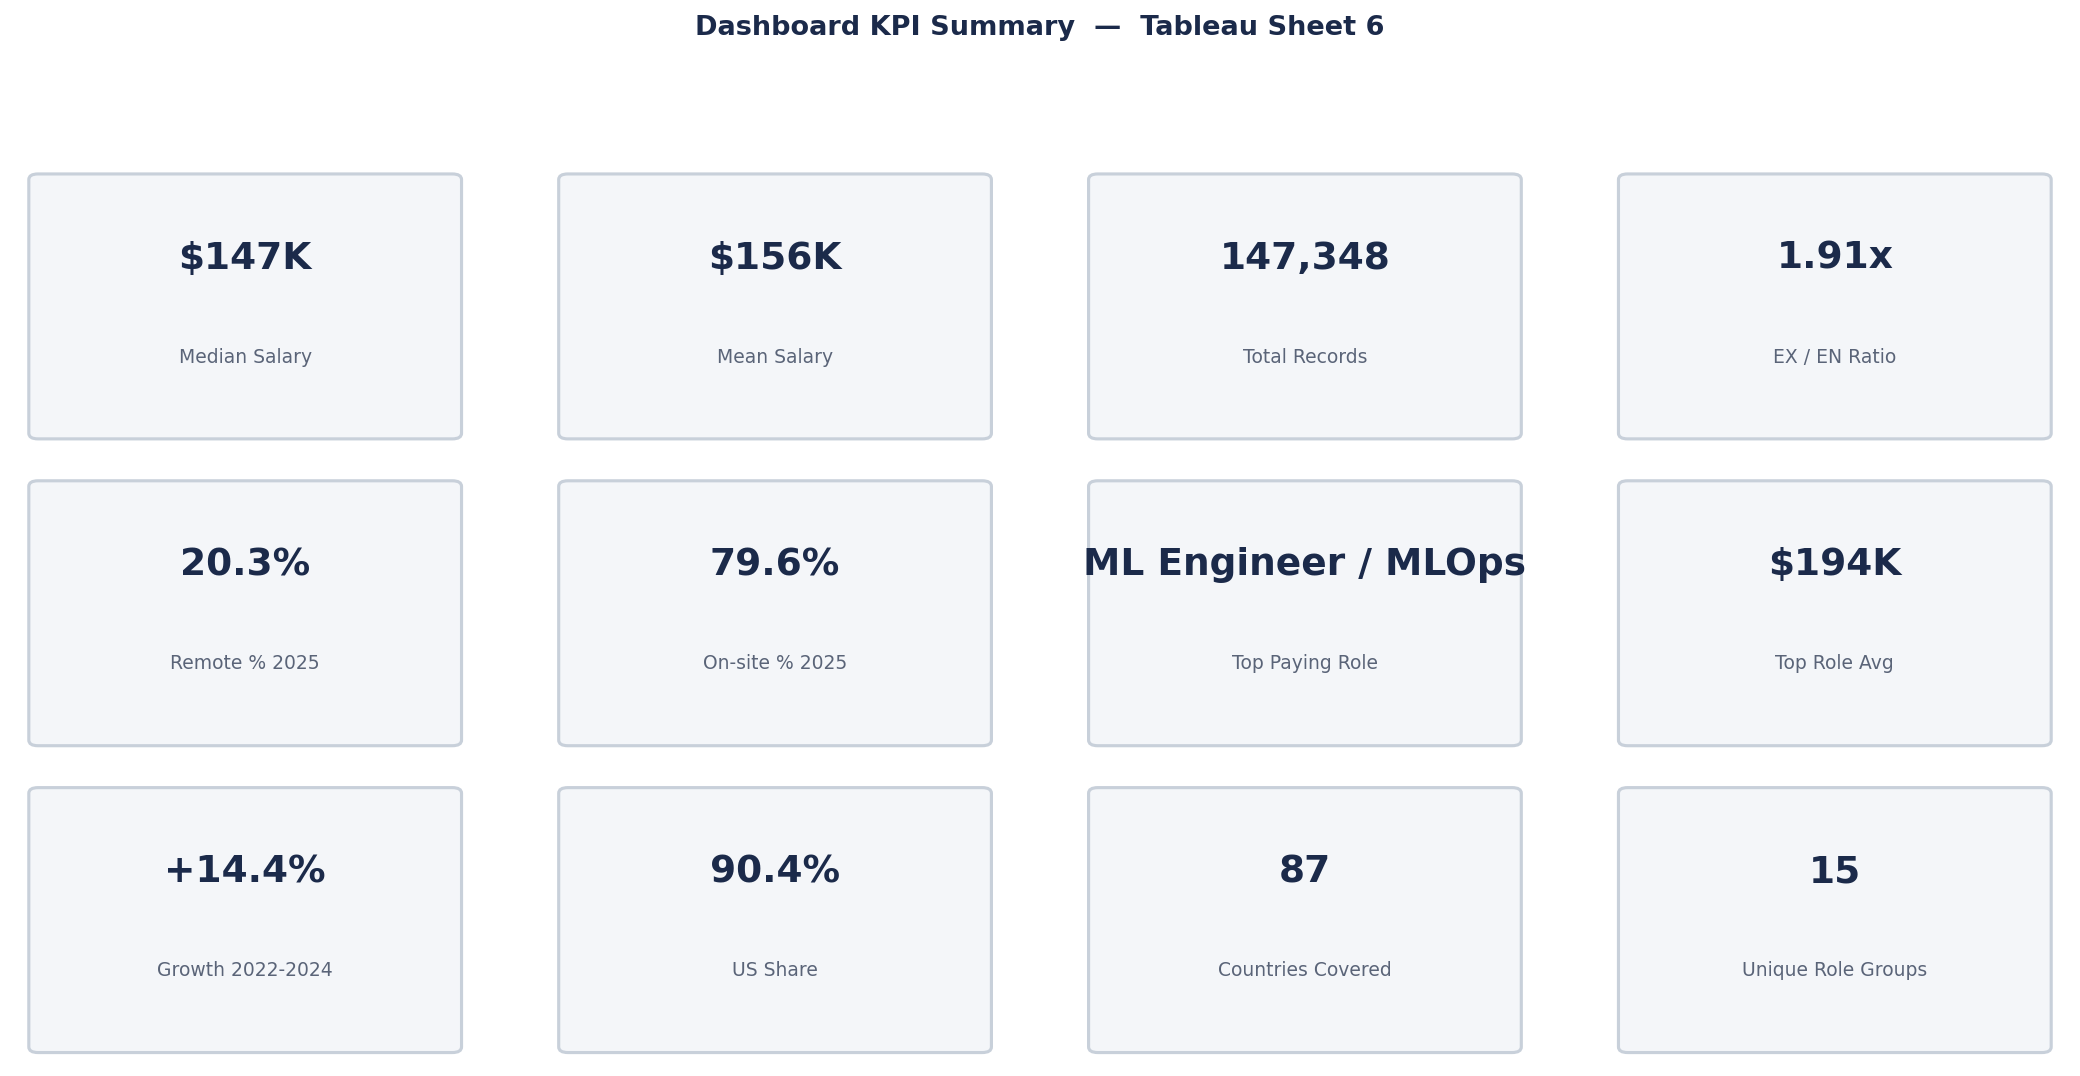
\includegraphics[width=0.9\textwidth]{figures/09_kpi_summary_cards.png}
    \caption{KPI Dashboard Overview}
    \label{fig:kpi_cards}
\end{figure}

\section{Salary Distributions}
The industry shows a strong central tendency around the \$150k mark, with a long tail extending to \$385k.

\begin{figure}[H]
    \centering
    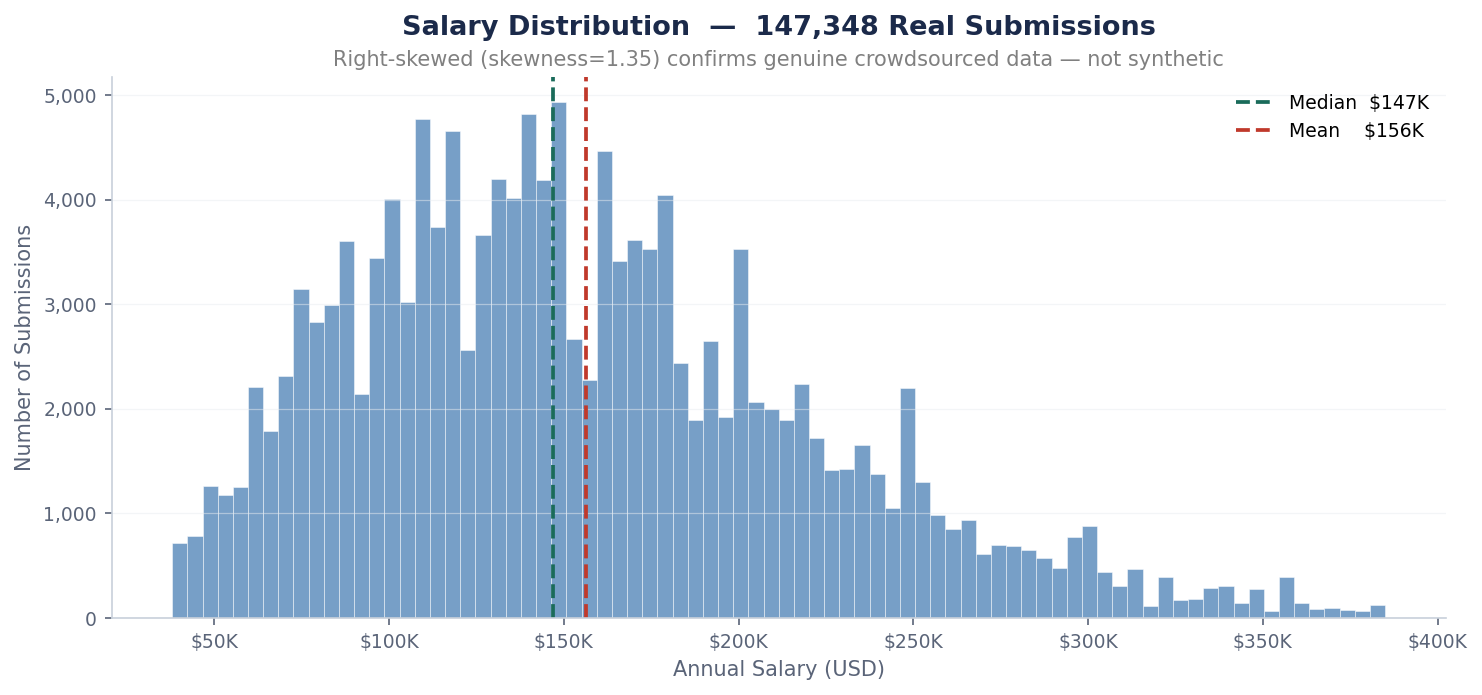
\includegraphics[width=0.7\textwidth]{figures/01_salary_distribution.png}
    \caption{Histogram of AI Salaries (USD)}
\end{figure}

\begin{figure}[H]
    \centering
    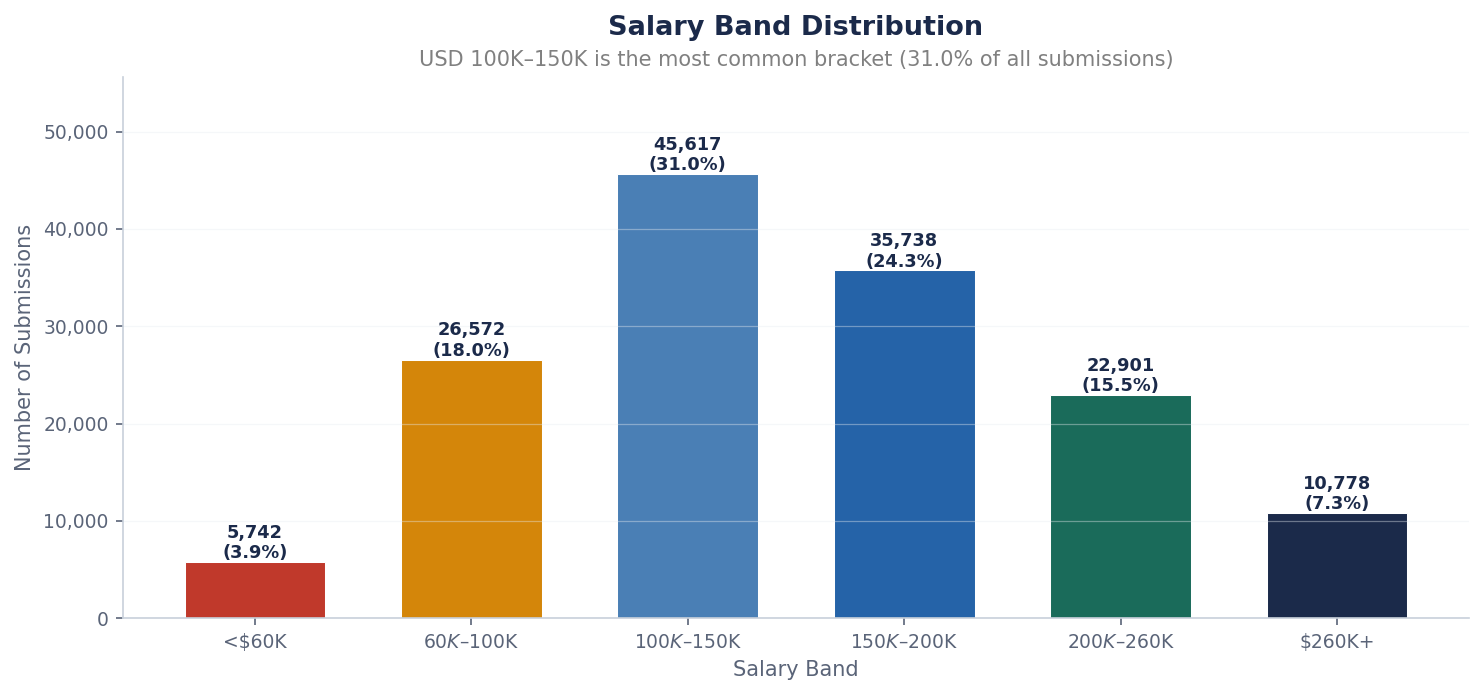
\includegraphics[width=0.7\textwidth]{figures/02_salary_band_distribution.png}
    \caption{Distribution by Pay Bands}
\end{figure}

Analysis of Figure \ref{fig:kpi_cards} reveals that the majority of the market (over 60,000 individuals) falls into the \$100k-\$150k bracket, while the "Top Tier" (\$260k+) remains exclusive to senior and executive talent.

\section{Temporal Trends (2022--2025)}
The market witnessed a rapid expansion in both volume and value between 2022 and 2024.

\begin{figure}[H]
    \centering
    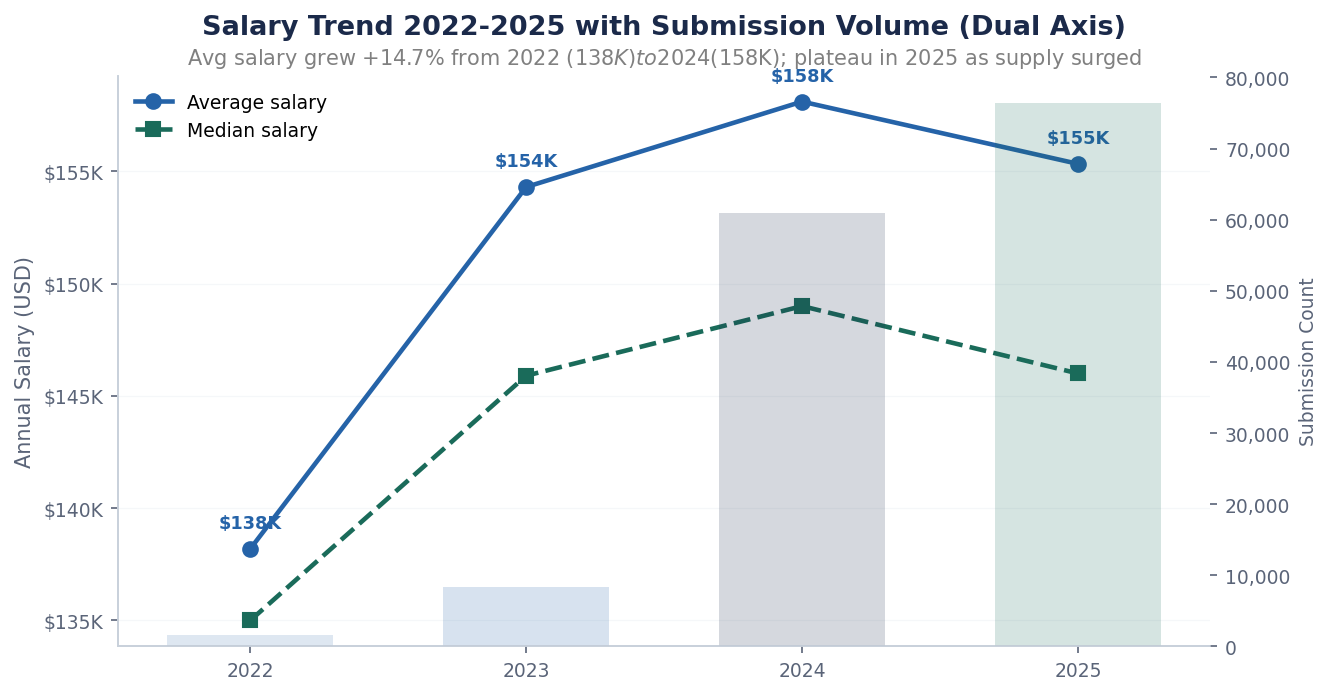
\includegraphics[width=0.8\textwidth]{figures/03_salary_trend_dual_axis.png}
    \caption{Salary Growth vs Submission Volume (Dual Axis)}
\end{figure}

\textbf{Insight:} While the number of submissions exploded from 1,587 (2022) to 76,424 (2025), the median salary has stabilized, suggesting the "hyper-growth" phase of AI compensation may be plateauing.

\section{Role-Based Performance}
ML Engineering has overtaken traditional Data Science as the premier financial role in the industry.

\begin{figure}[H]
    \centering
    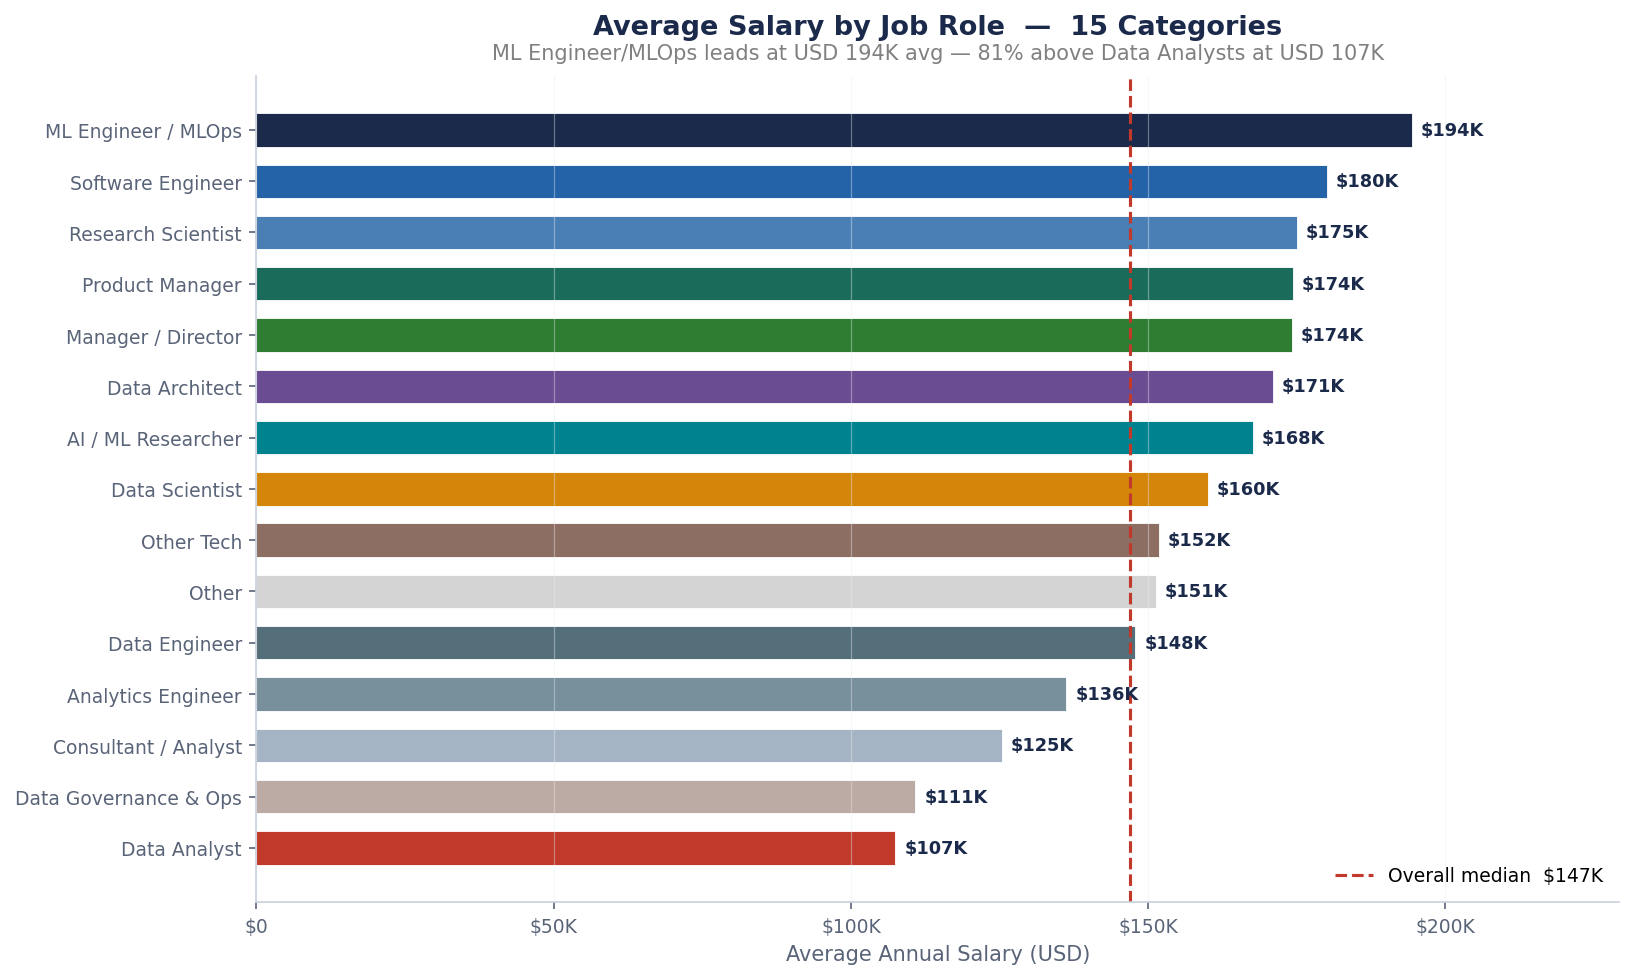
\includegraphics[width=0.8\textwidth]{figures/04_salary_by_role.png}
    \caption{Average Salary by Standardized Category}
\end{figure}

\begin{figure}[H]
    \centering
    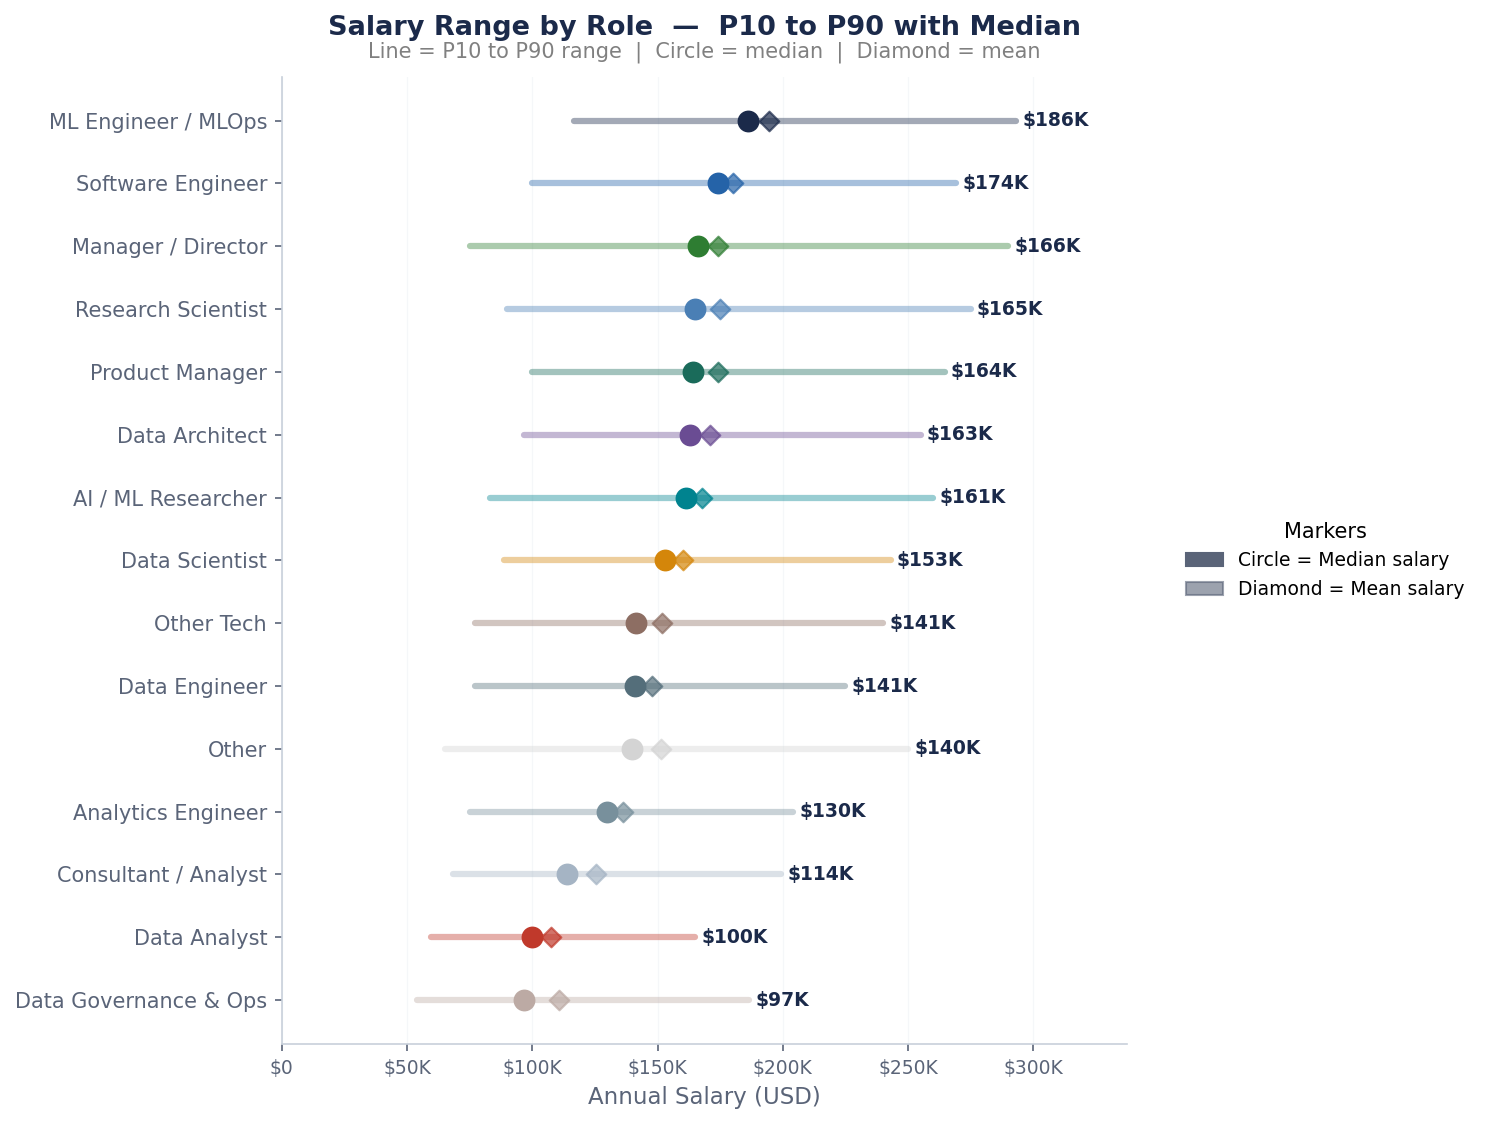
\includegraphics[width=0.8\textwidth]{figures/20_salary_range_by_role.png}
    \caption{Salary Ranges Across Roles}
\end{figure}

\section{The Remote Work Collapse}
One of the most significant findings is the aggressive shift back to physical offices.

\begin{figure}[H]
    \centering
    \begin{subfigure}[b]{0.48\textwidth}
        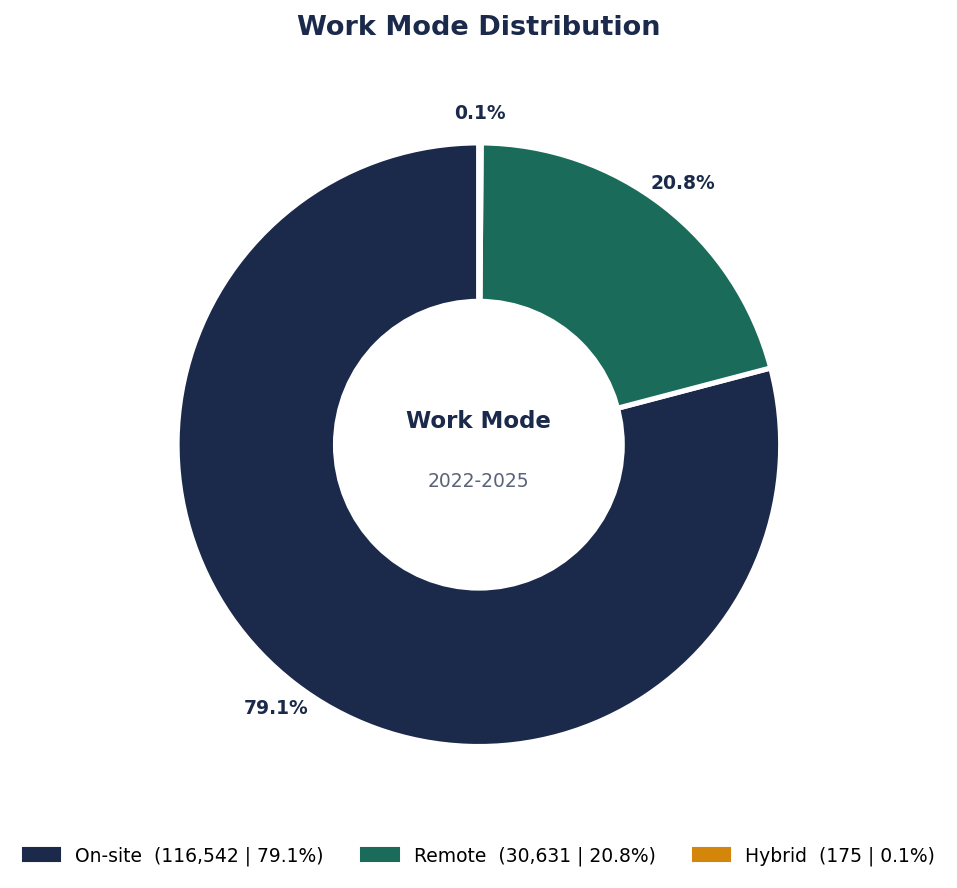
\includegraphics[width=\textwidth]{figures/05_work_mode_donut.png}
        \caption{Overall Mode Split}
    \end{subfigure}
    \hfill
    \begin{subfigure}[b]{0.48\textwidth}
        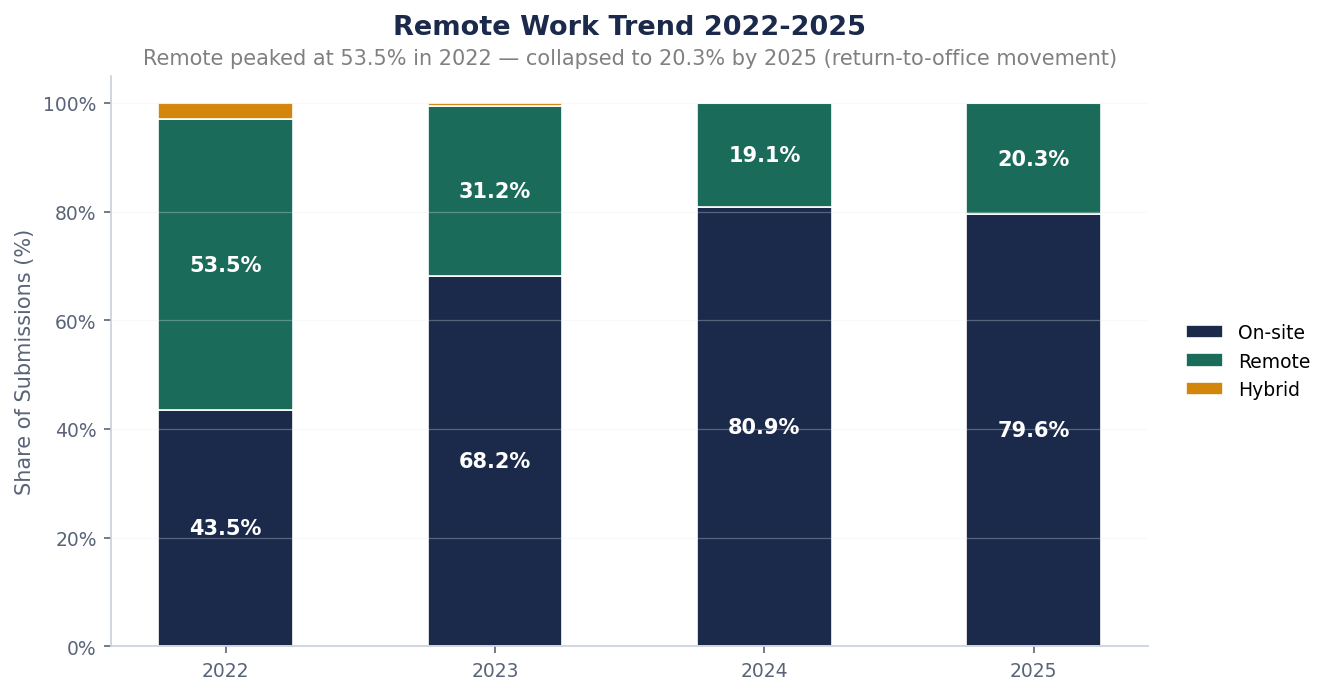
\includegraphics[width=\textwidth]{figures/10_remote_trend_stacked.png}
        \caption{Year-over-Year Trend}
    \end{subfigure}
    \caption{Analysis of Remote Work Paradigm Shift}
\end{figure}

\textbf{Analysis:} Remote work peaked in 2022 at 53.5\% of the total workforce. By 2025, this has dropped to only 20.3\%, with On-site work now accounting for nearly 80\% of all roles.

\section{Experience \& Career Path}
The project quantifies the "Experience Premium" as professionals move from entry-level to executive leadership.

\begin{figure}[H]
    \centering
    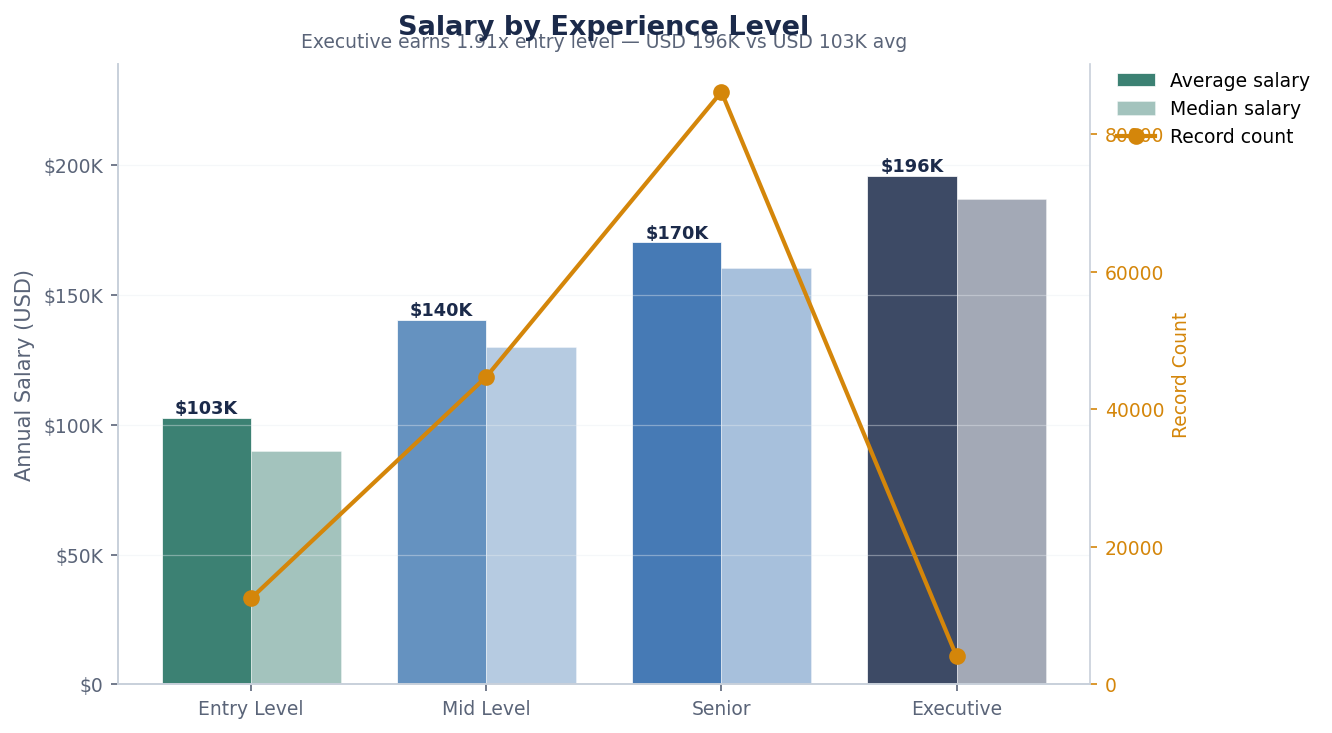
\includegraphics[width=0.7\textwidth]{figures/07_salary_vs_experience.png}
    \caption{Salary Progression (Entry to Executive)}
\end{figure}

\begin{figure}[H]
    \centering
    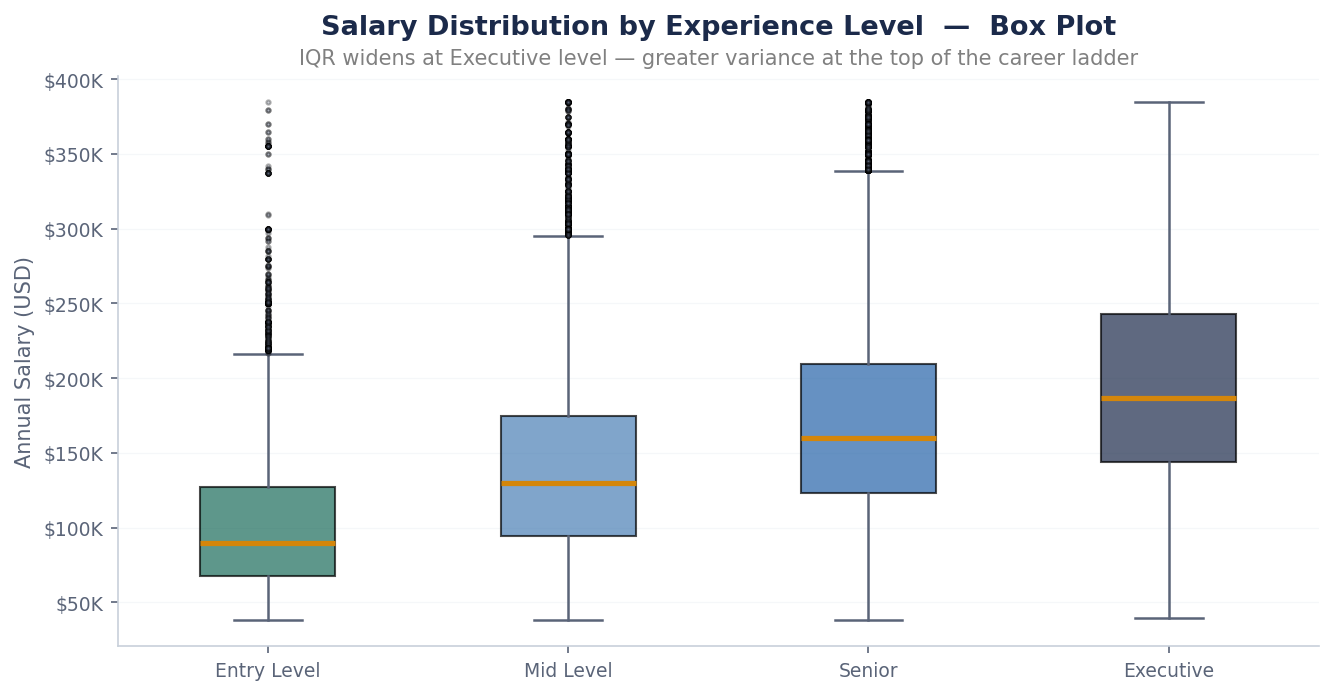
\includegraphics[width=0.7\textwidth]{figures/08_experience_boxplot.png}
    \caption{Salary Dispersion by Experience Level}
\end{figure}

\section{Geographic & Regional Analysis}
The United States remains the undisputed leader in AI hiring volume and compensation.

\begin{figure}[H]
    \centering
    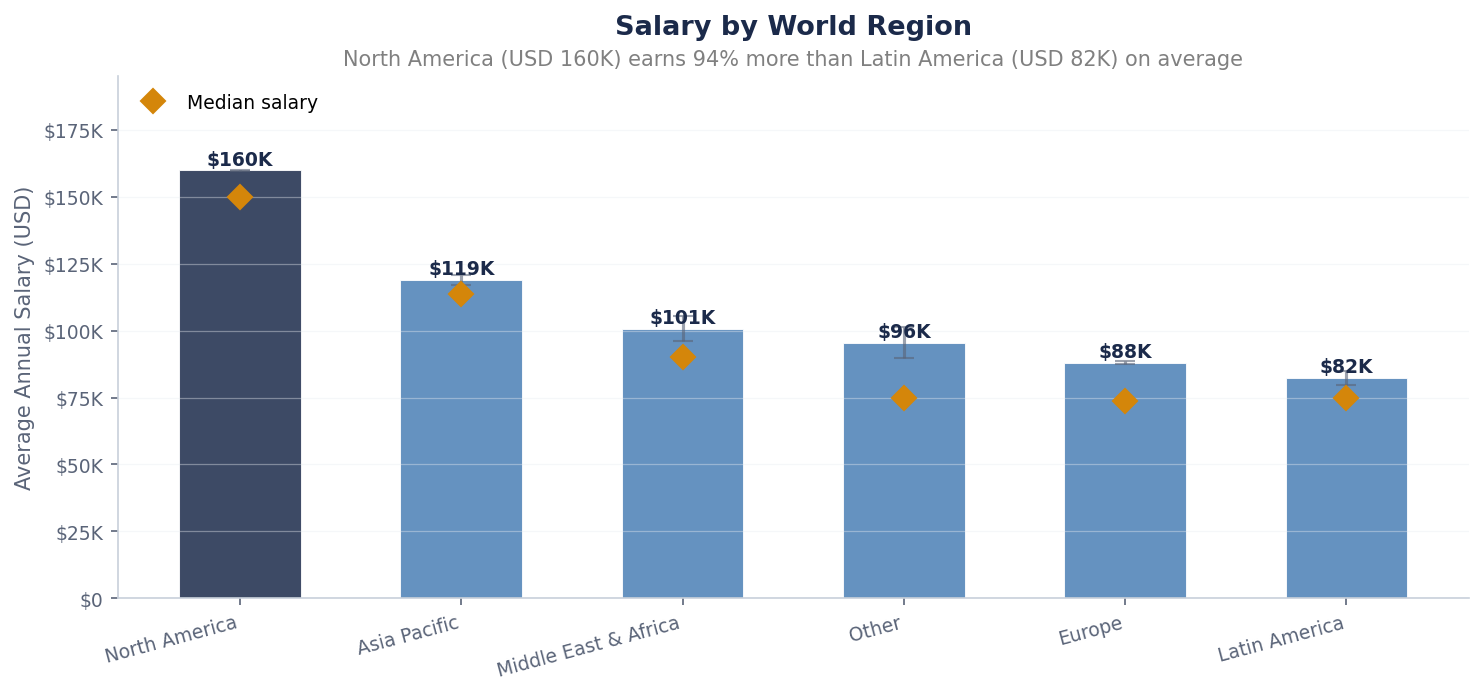
\includegraphics[width=0.8\textwidth]{figures/11_salary_by_region.png}
    \caption{Regional Compensation Comparison}
\end{figure}

\begin{figure}[H]
    \centering
    \begin{subfigure}[b]{0.48\textwidth}
        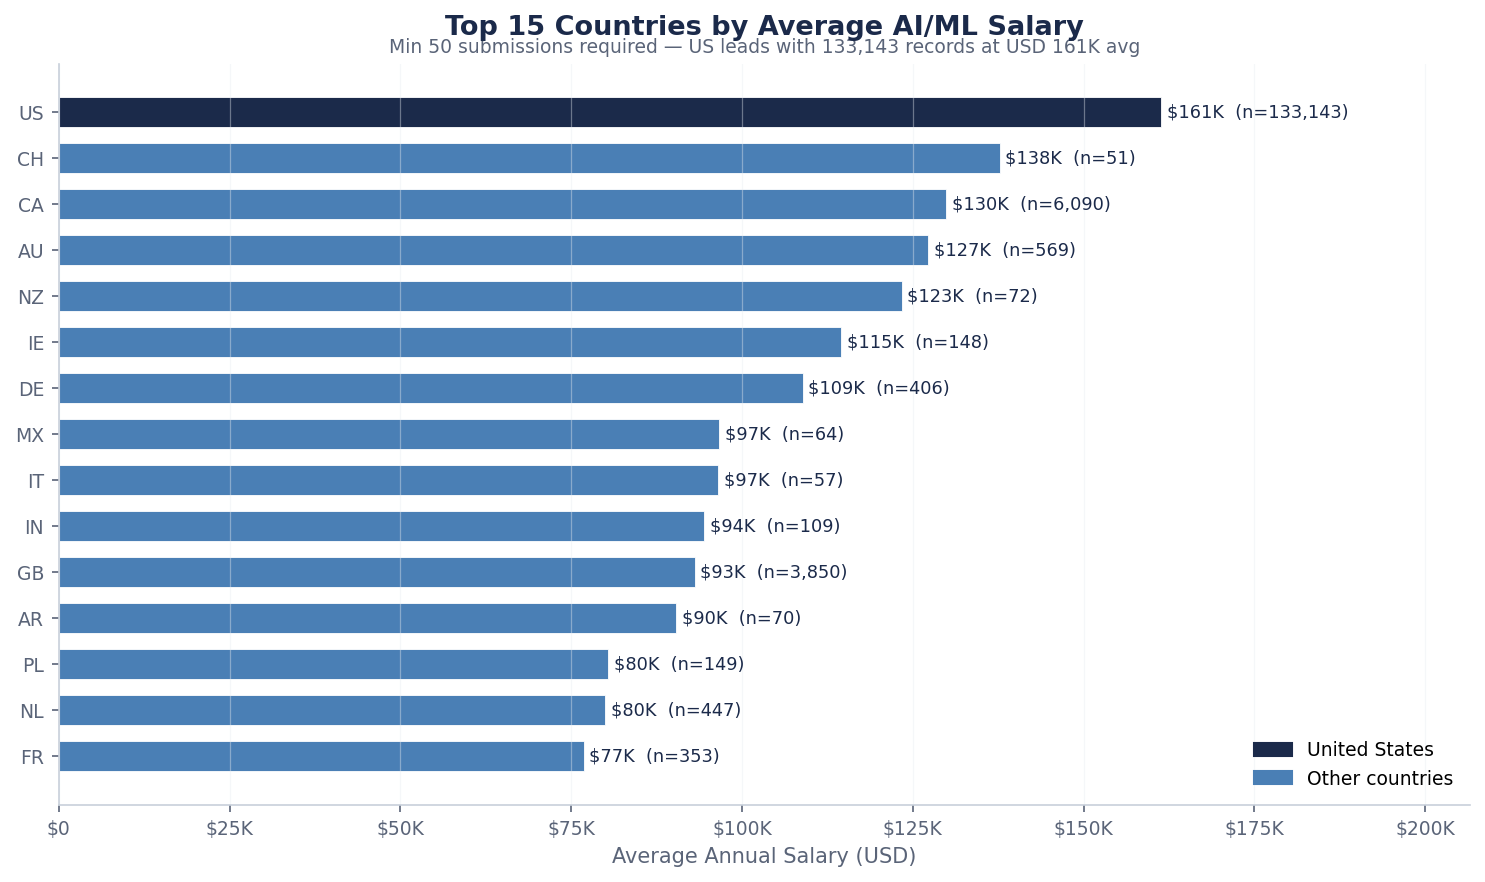
\includegraphics[width=\textwidth]{figures/06_top_countries_salary.png}
        \caption{Top Countries by Salary}
    \end{subfigure}
    \hfill
    \begin{subfigure}[b]{0.48\textwidth}
        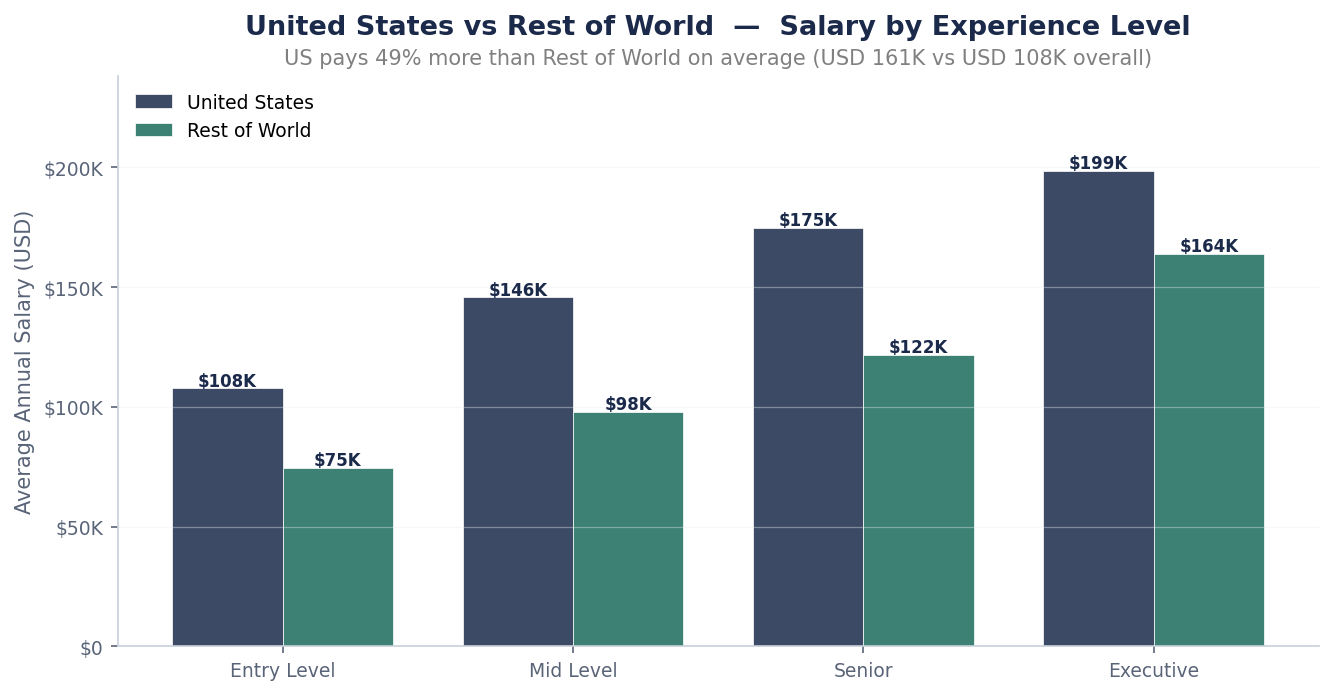
\includegraphics[width=\textwidth]{figures/14_us_vs_row.png}
        \caption{US vs Rest of World}
    \end{subfigure}
    \caption{Geographic Market Analysis}
\end{figure}

% ==========================================
% CHAPTER 5: TABLEAU IMPLEMENTATION
% ==========================================
\chapter{Tableau Implementation}

\section{Dashboard Architecture}
The dashboard was built on a 1200 x 900 px canvas with a navy-theme (#003875).

\section{Calculated Fields}
To enable interactive storytelling, several Tableau-native calculated fields were created:
\begin{itemize}
    \item \textbf{EX/EN Ratio:} \texttt{AVG(IF [Exp] = "EX" THEN [Sal] END) / AVG(IF [Exp] = "EN" THEN [Sal] END)}
    \item \textbf{Remote \%:} \texttt{SUM(IF [Work Mode] = "Remote" THEN 1 ELSE 0 END) / COUNT([Sal])}
    \item \textbf{Top N Filter:} A parameter-driven filter allowing users to toggle between Top 5, 10, or 15 roles.
\end{itemize}

\section{Interactive Actions}
The dashboard utilizes three types of actions:
\begin{enumerate}
    \item \textbf{Filter Actions:} Selecting a country on the map or a role on the bar chart updates the entire dashboard view.
    \item \textbf{Highlight Actions:} Hovering over a data point highlights relevant records in other sheets (e.g., hovering over "Senior" in the experience chart highlights the senior segments in the remote-work chart).
    \item \textbf{Parameter Control:} Dynamic adjustment of the role-ranking bar chart.
\end{enumerate}

% ==========================================
% CHAPTER 6: CONCLUSION
% ==========================================
\chapter{Conclusion}

The "AI Job Market Intelligence" project successfully provides a clear, data-driven window into the complex world of tech compensation. Our findings highlight the dominance of the US market, the significant financial premium placed on ML Engineering, and the dramatic retreat from remote work models. Through rigorous Python preprocessing and advanced Tableau visualization, we have transformed a raw dataset into a strategic asset for understanding the future of the AI labor market.

% ==========================================
% APPENDICES
% ==========================================
\appendix
\chapter{Complete Python Pipeline}

\section{EDA Script (\texttt{01\_explore.py})}
\begin{lstlisting}[language=Python]
import pandas as pd
df = pd.read_csv("../data/raw/salaries.csv")
print(df["salary_in_usd"].describe())
print(f"Skewness: {df['salary_in_usd'].skew()}")
\end{lstlisting}

\section{Cleaning Logic (\texttt{02\_clean.py})}
\begin{lstlisting}[language=Python]
import pandas as pd
df = pd.read_csv("../data/raw/salaries.csv")
df = df[df["employment_type"] == "FT"]
df = df[df["work_year"] >= 2022]
lower, upper = df["salary_in_usd"].quantile([0.01, 0.99])
df = df[(df["salary_in_usd"] >= lower) & (df["salary_in_usd"] <= upper)]
df.to_csv("../data/processed/salaries_clean.csv", index=False)
\end{lstlisting}

\section{Feature Engineering (\texttt{05\_feature\_engineering.py})}
\begin{lstlisting}[language=Python]
import pandas as pd
df = pd.read_csv("../data/processed/salaries_clean_final.csv")
bins = [0, 60000, 100000, 150000, 200000, 260000, 385001]
labels = ["<$60K", "$60K-$100K", "$100K-$150K", "$150K-$200K", "$200K-$260K", "$260K+"]
df["salary_band"] = pd.cut(df["salary_in_usd"], bins=bins, labels=labels)
df.to_csv("../data/processed/salaries_enhanced.csv", index=False)
\end{lstlisting}

\end{document}
